\documentclass[tikz,border=8pt]{standalone}

% общий стиль (подключается через TEXINPUTS)
% tikz-style.tex (общий стиль для всех TikZ-картинок)
\RequirePackage[T1,T2A]{fontenc}
\RequirePackage[utf8]{inputenc}

% Palatino-подобный шрифт (как в MathJax часто воспринимается «более вытянутым»)
\RequirePackage{txfonts}
% txfonts даёт предупреждение по кириллице (T2A/txr не определён).
% Оставляем txfonts для математики, а текстовый шрифт возвращаем на Computer Modern,
% чтобы не искать T2A/txr и убрать предупреждения.
\renewcommand{\rmdefault}{cmr}
\renewcommand{\sfdefault}{cmss}
\renewcommand{\ttdefault}{cmtt}

\RequirePackage{tikz}
\RequirePackage{xcolor}
\usetikzlibrary{calc}

% цвета
\definecolor{lightgreen}{RGB}{214,234,214}
\definecolor{darkgreen}{HTML}{0B7A0B}
\definecolor{darkred}{HTML}{DF0000}

\definecolor{midgreen}{HTML}{2E9B2E}
\definecolor{palegreen}{RGB}{235,246,235}
\definecolor{olivegreen}{HTML}{3E6B2F}

\definecolor{lightred}{RGB}{255,220,220}
\definecolor{midred}{HTML}{E04545}
\definecolor{darkred2}{HTML}{A80000}

\definecolor{lightblue}{RGB}{220,232,255}
\definecolor{midblue}{HTML}{2E5BD6}
\definecolor{darkblue}{HTML}{0B2E8A}

\definecolor{lightgray}{RGB}{240,240,240}
\definecolor{midgray}{RGB}{170,170,170}
\definecolor{darkgray}{RGB}{80,80,80}

\definecolor{vtxfill}{RGB}{86,193,255}
\definecolor{vennfill}{RGB}{220,232,255}


% единый набор стилей TikZ
\tikzset{
    lab/.style={
        font=\fontsize{24}{32}\selectfont
    }
}

% local fallback: tikz-style defines darkred/darkgreen, but darkblue may be absent

\usepackage{tikz}
\usetikzlibrary{arrows.meta,positioning}

\begin{document}
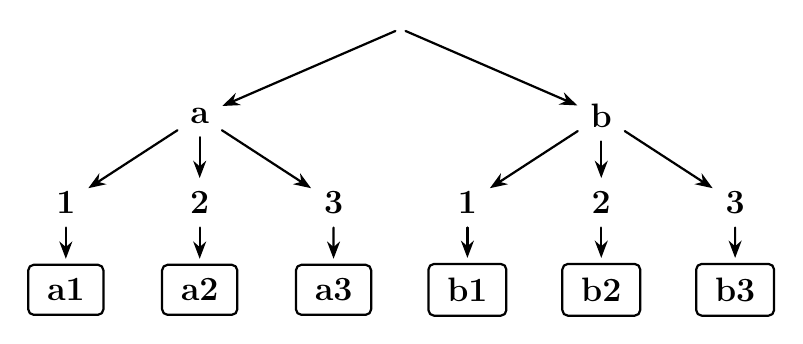
\begin{tikzpicture}[
  line cap=round,
  line join=round,
  scale=0.85,
  transform shape,
  grow=down,
  level distance=13mm,
  edge from parent/.style={draw=black, -{Stealth[length=2.2mm]}, line width=0.8pt, shorten >=2.0pt, shorten <=2.0pt},
  every node/.style={font=\bfseries\Large, align=center},
  every leaf/.style={font=\bfseries\Large},
  level 1/.style={sibling distance=60mm},
  level 2/.style={sibling distance=20mm},
  level 3/.style={sibling distance=13mm},
  level 4/.style={sibling distance=13mm, level distance=13mm}
]

% ---------- node styles ----------
\tikzset{
  labelNode/.style={font=\bfseries\Large, text=black},
  numNode/.style={font=\bfseries\Large, text=black},
  word/.style={font=\bfseries\Large, text=black, draw=black, rounded corners=2pt, inner xsep=8pt, inner ysep=6pt}
}

% ---------- hanging tree (black) ----------
\node[coordinate] {}
  child { node[labelNode] {a}
    child { node[numNode] {1}
      child { node[word] {a1} }
    }
    child { node[numNode] {2}
      child { node[word] {a2} }
    }
    child { node[numNode] {3}
      child { node[word] {a3} }
    }
  }
  child { node[labelNode] {b}
    child { node[numNode] {1}
      child { node[word] {b1} }
    }
    child { node[numNode] {2}
      child { node[word] {b2} }
    }
    child { node[numNode] {3}
      child { node[word] {b3} }
    }
  };

\end{tikzpicture}
\end{document}